\documentclass[10pt,twocolumn,letterpaper]{article}

\usepackage{cvpr}
\usepackage{times}
\usepackage{epsfig}
\usepackage{graphicx}
\usepackage{amsmath}
\usepackage{caption}
\usepackage{subcaption}
\usepackage{booktabs}
\usepackage{amssymb}
%\usepackage{hyperref}

% Include other packages here, before hyperref.

% If you comment hyperref and then uncomment it, you should delete
% egpaper.aux before re-running latex.  (Or just hit 'q' on the first latex
% run, let it finish, and you should be clear).
\usepackage[breaklinks=true,bookmarks=false]{hyperref}

\cvprfinalcopy % *** Uncomment this line for the final submission

\def\cvprPaperID{****} % *** Enter the CVPR Paper ID here
\def\httilde{\mbox{\tt\raisebox{-.5ex}{\symbol{126}}}}

% Pages are numbered in submission mode, and unnumbered in camera-ready
%\ifcvprfinal\pagestyle{empty}\fi
%\setcounter{page}{4321}
\begin{document}

%%%%%%%%% TITLE
\title{Assignment 2: Adaboost}

\author{Moaz Mohamed\\
The University of Adelaide\\
Adelaide SA 5005\\
{\tt\small a1779177@student.adelaide.edu.au}
% For a paper whose authors are all at the same institution,
% omit the following lines up until the closing ``}''.
% Additional authors and addresses can be added with ``\and'',
% just like the second author.
% To save space, use either the email address or home page, not both

}

\maketitle
%\thispagestyle{empty}

%%%%%%%%% ABSTRACT
%\begin{abstract}
  % The ABSTRACT is to be in fully-justified italicized text, at the top
  % of the left-hand column, below the author and affiliation
  % information. Use the word ``Abstract'' as the title, in 12-point
  % Times, boldface type, centered relative to the column, initially
  % capitalized. The abstract is to be in 10-point, single-spaced type.
  % Leave two blank lines after the Abstract, then begin the main text.
 %  Look at previous CVPR abstracts to get a feel for style and length.
%\end{abstract}

%%%%%%%%% BODY TEXT
\section{Introduction}

Over the last few years, Machine learning had a significant impact in the current technological landscape. 
The application of numerous Deep learning algorithms have been implemented in different sectors. In this paper Adaboost algorithm will be explored and its performance will be investigated on classification task on the provided dataset.In addition to a complete review of the Adaboost algorithm describing its strength and weakness.
%-------------------------------------------------------------------------
\section{Methodology and Background}



\subsection{AdaBoost}

Boosting is the idea of utilizing the a number of weak learner and combine them to make a strong learner that is capable of reaching a training error of zero, hence a weak learner alone is able to reach zero training error. instead of using a strong learner like Support Vector machine (SVM) adaboost is an ensemble of weighted weak learners Eq (\ref{eq:ada_en}).



\begin{equation}
H(x)=\operatorname{sign}\left(\sum_{t=1}^{T} \alpha_{t} h_{t}(x)\right)
\label{eq:ada_en}
\end{equation}


Some learners do preform better than others, hence the weighting is depended on the accuracy of the learner.

\begin{equation}
\alpha_{t}=\frac{1}{2} \ln \left(\frac{1-\epsilon_{t}}{\epsilon_{t}}\right)
\label{eq:alpha}
\end{equation}

In every new iteration a new weak leaner is used to minimize the error of Eq \ref{ed_err}. in addition to a weight matrix for the contribution of error for every data point. which increase and decreses for every data point per iteration Eq \ref{eg:w_err}

\begin{equation}
\epsilon_{t}=\sum_{i=1}^{n} \mathbf{1}\left[h_{t}\left(x_{i}\right) \neq y_{i}\right] w_{i}^{(t)}
\label{ed_err}
\end{equation}


\begin{equation}
w_{i}^{(t+1)}=w_{i}^{(t)} \cdot e^{-\alpha^{t} y_{i} h_{t}\left(x_{i}\right)}
\label{eg:w_err}
\end{equation}

\subsection{Weak Learner}
A weak learner can be any learner that is better than a coin tossing. Decision stumps have been used as a weak learner in most Adaboost implementations. Decision stumps can be treated as decision trees with max depth of 1 , increasing the depth of the tree can be used to study the affect of having stronger learner in Adaboost algorithm. Decision stumps can also be implemented as using greedy search to test different unique values in each feature in the dataset to come up with the best threshold for the split. in this project sklearn implementation has been used for ease of use and the added benefit of using optimized code to run multiple runs of experiments efficiently. 

\section{Experimental Analysis.}

\subsection{Training and Testing Curves}
in figure \ref{fig:tr vs te}. Adaboost reaches a high accuracy in relatively small number of iteration. that is due to the weighting in Eq \ref{eq:alpha}. As high weighting is applied to the first learners especially with the learners with low error or loss and as the boosting continues $\alpha_{t}$ gets smaller and smaller as the contribution of additional learners gets smaller and hence why Adaboost tends not to overfit easily. even with increasing the weak leaner ( decision stumps ) depth to 3. the training accuracy increases faster than depth of 1 while not showing any signs of overfitting. hence Adaboost does fix the successfully combines classifiers with high bias ( decision stumps ) and at the same time has an inbuilt feature of combating overfitting.

  

\begin{figure}[htb]
  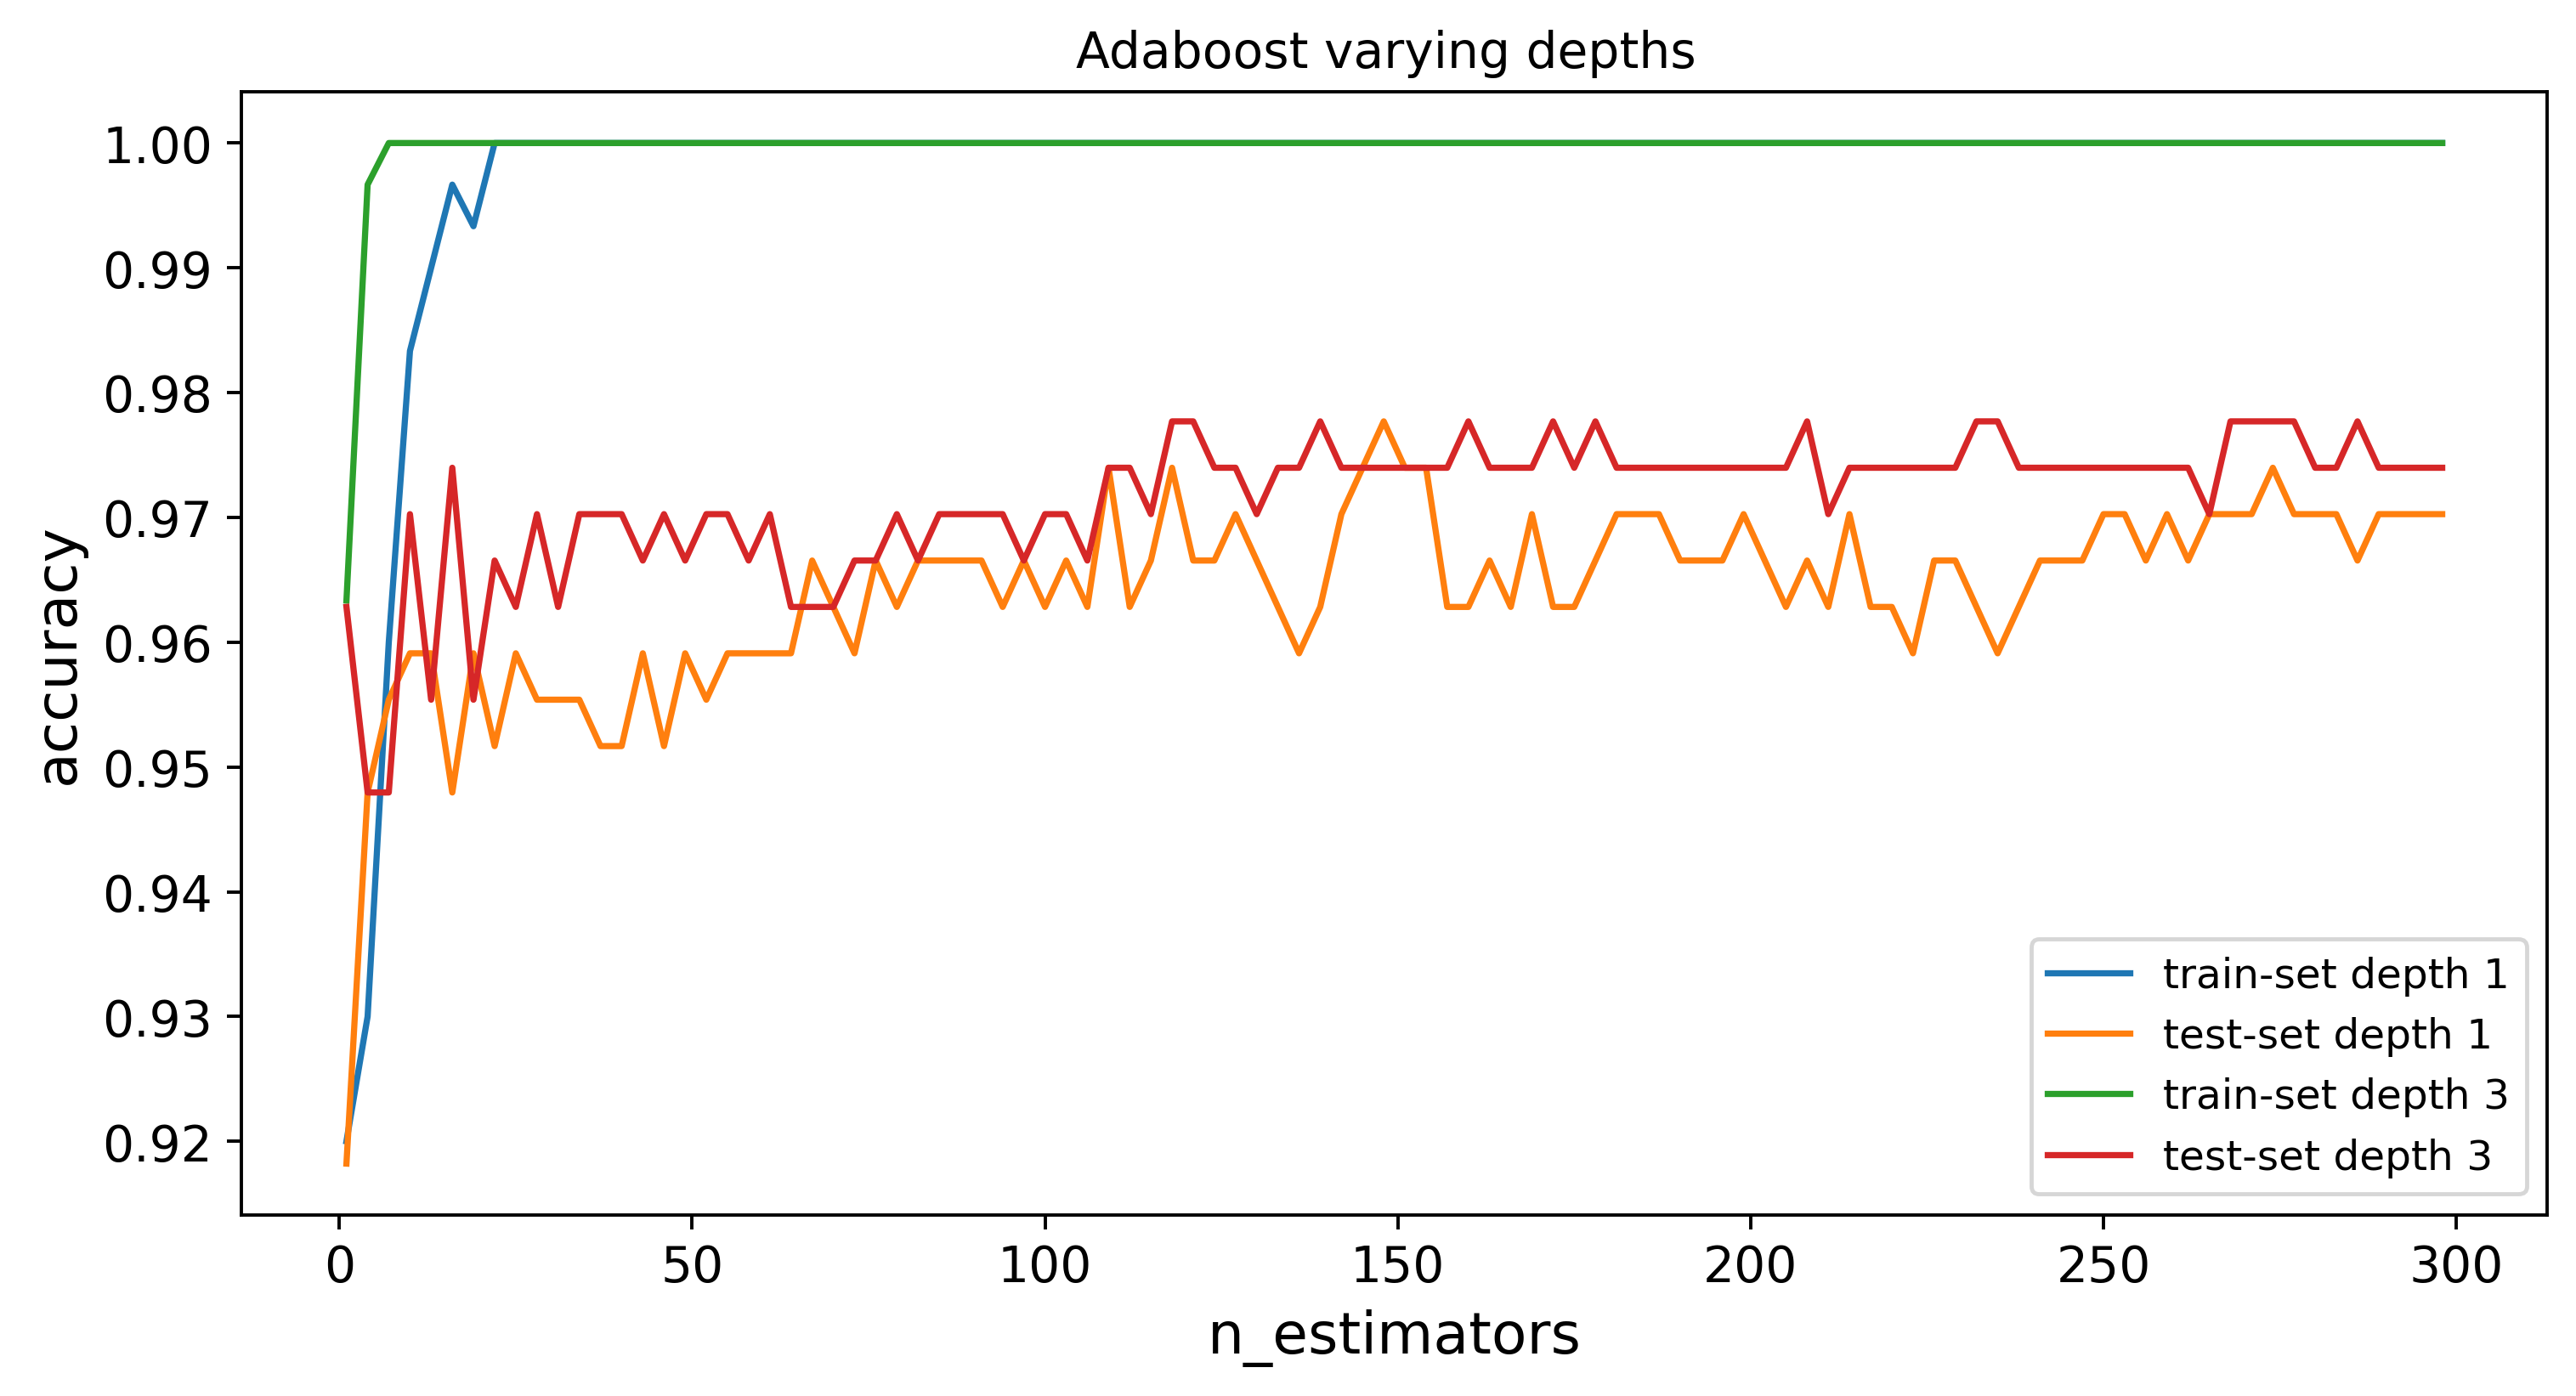
\includegraphics[width=\linewidth]{Adaboost_depth_2.png}A weak learner can be any learner that is better than a coin tossing. Decision stumps have been used as a weak learner in most Adaboost implementations. Decision stumps can be treated as decision trees with max depth of 1 , increasing the depth of the tree can be used to study the affect of having stronger learner in Adaboost algorithm. Decision stumps can also be implemented as using greedy search to test different unique values in each feature in the dataset to come up with the best threashold for the spilt 

  \caption{Training vs testing}
  \label{fig:tr vs te}
\end{figure}

\vspace{3.00mm} 







\subsection{Performance on provided data-set}
In table \ref{tab:results} Adaboost does outperform SVM without and with no regularization. there are certain advantageous that goes Adaboost an edge. Adaboost makes no assumptions about the data but in SVM since the objective is finding the largest margin. hence feature vectors with high values can hinder SVM ability to find the margin while in Adaboost that isn't a problem. the mentioned Adaboost algorithm is sensitive to noise. as in Eq \ref{eg:w_err} for noisy datasets the weight for the misclassified data points will keep increasing and new learner will try to classify such points correctly but in SVM regularization parameter can be adjusted to cater for the inherit noise in the dataset. 



\begin{table}[htb]
\centering
\begin{tabular}{|l|l|l|l|} 
\toprule
Algorithm            & accuracy  \\ 
\hline
Adaboost scratch     & 96.282\%      \\ 
\hline
Adaboost sklearn     & 96.654\%      \\ 
\hline
SVM-C=0              & 95.539\%      \\
\hline
SVM-C=1000           & 97.026\%      \\
\bottomrule
\end{tabular}
\caption{SVM vs Adaboost}
\label{tab:results}
\end{table}





\section{Conclusion}

From bias and variance prospective. Adaboost can be seen as method to take an ensemble of high bias learners combine them is such way to decrease the bias and increase the variance by adding learners and yet not overfit easily. Of-course no algorithm is perfect. due to Eq \ref{eg:w_err} Adaboost will have such emphases on the misclassified data points and for each iteration will try to adjust the decision boundary to correctly classify every data point correctly. 


%\bibliography{egbib.bib} 
%\bibliographystyle{ieeetr}

\end{document}
